\documentclass[12px, a4paper]{article}
\usepackage[margin=50pt]{geometry}
\usepackage{graphicx}
\graphicspath{ {./images} }
\title{Preserving Accents in Real-Time Audio Translation: A Novel Approach for Linguistic Fidelity}
\author{Irfan Wani - Lovely Professional University}
\date{25 April 2024}
\begin{document}    
\maketitle
    \begin{abstract}
    Our system takes the audio as input and translates it into the target language in real-time. Audio files can also be used as input for the program and it will provide the reuslt in the desired language. The system is based on the concept of real-time audio translation. The system works in multiple steps, starting with taking the input from the user (primarily in english or detecting the language of the audio), converting the audio to text, taking the target language as the input from the user (like Hindi, Arabic etc) and then translating the text to the target language. Another step is the reverse of the previous steps where the text is converted back to audio and then played on the device.  NLP (Natural Language Processing) comes into play to make the whole thing work. NLP helps in translation, where it checks the grammer, words etc to make sure the translated text makes sense.
    The last step utilizes text-to-speech (TTS) models. These models are trained on audio recordings of different people speaking with different voices and tones, along with the corresponding input text. These models learn the characteristics of a particular voice, like pitch, timbre, and inflection. Then, when we provide some different text as input, they can synthesize speech that sounds like the target voice. Some AI systems can even adjust the synthesized speech to match the emotional tone of the original audio.
    \end{abstract}
    \textbf{Keywords: } NLP, Real-Time Audio Translation, Accents, Linguistic Fidelity, Google Translator AI, Whisper AI, Text-To-Speech.
\section{Introduction}
Talking about the realtime audio translation, it is a process where the audio is converted to text and then the text is translated to the target language. The process is done in real-time and the user can speak in the target language and the system will translate it to the target language. It is used in different fields like audio translation apps, language learning apps, audio caption generators etc. The input can be from a user in real time or from an audio file. The different steps involved in the process are:
\begin{enumerate}
    \item Taking the input from the user in realtime or using an input audio file. In this project, speech recognition package has been used to either read an audio file or to take the input from the user in real time by using the Microphone() class.
    \item Detecting the audio language. Speech recognition package has support for multiple models to detect the language of the audio. In this project, the model used is the Whisper model by Open AI.
    \item Converting the audio to text. The audio is converted to text using the Whisper model.
    \item Destination language is taken from the user to which the input audio will be translated. This is done by the same process.
    \item Using the Translator from googletrans package which provides the free Google Translation API for python, the input text is translated to the target language.
    \item Google Text to Speech is used to create an audio file which contains the translated text in the desired language.
    \item The audio file is played on the device using the playaudio package.
    \item  Text-to-speech (TTS) models are utilized that are trained on audio recordings of different speeches, along with the corresponding text. After learning different characteristics of the speeches, these models try to synthesize speech that sounds like the target voice. Some AI systems can even adjust the synthesized speech to match the emotional tone of the original audio.
    
\end{enumerate}
\textbf{Model used:}
The model used in this project is Whisper AI from Open AI. Whisper is a general-purpose speech recognition model. It is trained on a large dataset of diverse audio and is also a multitasking model that can perform multilingual speech recognition, speech translation, and language identification.
\section{Literature Review}
In current time, Real-time audio translation has become increasingly prevalent with the rise of globalization and the latest technologies. The ability to translate spoken language, especially in real-time, has revolutionized communication across geographical and linguistic barriers. 

Core Components of Audio Translation are:

\textbf{Automatic Speech Recognition (ASR)}: This technology converts spoken audio into text format. ASR systems are trained on vast amounts of speech data to recognize phonemes (basic units of sound) and translate them into words. Accuracy is crucial for effective translation, as errors in ASR can significantly impact the final output. Recently, the speech community is seeing a significant trend of moving from deep neural network based hybrid modeling to end-to-end modeling (often read as E2E modeling) for automatic speech recognition (ASR). While End to End models achieve the desired results in most benchmarks in terms of ASR accuracy, the use of hybrid models is still on top of commercial ASR systems at the current time. There are lots of practical factors that affect the production model deployment decision. Traditional hybrid models, being optimized for production for decades, are usually good at these factors. (e.g., [Jinyu Li] (2021))

\textbf{Machine Translation (MT)}: This technology translates text from one language to another. Statistical or neural MT models analyze the source text, considering grammar, syntax, and context, to generate the target language translation. The quality of MT models significantly impacts the fluency and accuracy of the translated audio. Large Language Models (LLM) have demonstrated their strong ability in the field of machine translation (MT), yet they suffer from high computational cost and latency. Therefore, the transfer of translation knowledge from giant LLMs to medium-sized machine translation models is a promising research direction. However, traditional knowledge distillation methods doesn't take the capability of student and teacher models into consideration, therefore student models are taught repeatedly on the knowledge they have learned, thus failing to reach the desired results. (e.g., [Jiahuan Li, Shanbo Cheng, Shujian Huang, Jiajun Chen] (2024))

\textbf{Text-to-Speech (TTS)}: This technology synthesizes speech from written text. TTS systems are trained on audio recordings of human speech paired with corresponding text. They learn the characteristics of human voice, such as pitch, intonation, and rhythm, to generate natural-sounding speech in the target language. Non-autoregressive text to speech (TTS) models such as FastSpeech can synthesize speech significantly faster than previous autoregressive models with comparable quality. (e.g., [Yi Ren, Chenxu Hu, Xu Tan, Tao Qin, Sheng Zhao, Zhou Zhao, Tie-Yan Liu] (2021)) \linebreak\linebreak
\textbf{Recent Advancements}

\textbf{End-to-End Speech-to-Speech Translation (ST)}: This approach combines ASR, MT, and TTS into a single system, streamlining the translation process. Recent research by [Biao Zhang, Barry Haddow, Rico Sennrich] (2022) demonstrates promising results in terms of efficiency and fluency.

\textbf{Neural Machine Translation (NMT)}: NMT models utilize deep learning architectures to achieve superior translation accuracy compared to traditional statistical methods. Research by [Dzmitry Bahdanau, Kyunghyun Cho, Yoshua Bengio] (2016) explores the application of NMT for audio translation, achieving significant improvements in fluency and grammatical correctness. Neural machine translation(NMT) is a recently proposed approach to machine translation. Unlike the traditional statistical machine translation, the neural machine translation aims at building a single neural network that can be jointly tuned to maximize the translation performance. The models proposed recently for neural machine translation often belong to a family of encoder-decoders and consists of an encoder that encodes a source sentence into a fixed-length vector from which a decoder generates a translation.

\textbf{Speaker Diarization and Adaptation}: These techniques identify and separate speech from different speakers within an audio recording. This allows for speaker-specific translation, particularly beneficial in conference settings. [Tae Jin Park, Naoyuki Kanda, Dimitrios Dimitriadis, Kyu J. Han, Shinji Watanabe, Shrikanth Narayanan] (2021) propose a diarization-based approach for real-time multi-speaker translation. Speaker diarization is a task to label audio or video recordings with classes that correspond to speaker identity, or in short, a task to identify "who spoke when". In the early years, speaker diarization algorithms were developed for speech recognition on multispeaker audio recordings to enable speaker adaptive processing. These algorithms also gained their own value as a standalone application over time to provide speaker-specific metainformation for downstream tasks such as audio retrieval. More recently, with the emergence of deep learning technology, which has driven revolutionary changes in research and practices across speech application domains, rapid advancements have been made for speaker diarization. \linebreak\linebreak

\begin{figure}[!htb]
    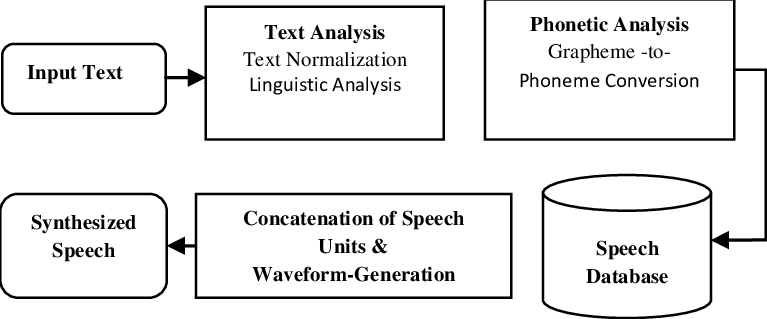
\includegraphics[width=\textwidth]{texttospeech.png}
    \caption{Block diagram of Text-to-Speech System Techniques of speech synthesis}
\end{figure}

\textbf{Challenges and Future Directions}

\textbf{Accuracy and Fluency}: Balancing accuracy in meaning preservation with natural-sounding fluency remains a challenge. Future research should focus on improving the robustness of ASR and NMT models to handle diverse speaking styles and background noise.

\textbf{Preserving Speaker Identity}: Current systems often lose speaker-specific characteristics like accent and intonation during translation. Research by [Sameen Maruf, André F. T. Martins, Gholamreza Haffari] (2019) explores accent-aware NMT to preserve speaker identity, paving the way for more nuanced translations. Despite the progress made in sentence-level NMT, current systems still fall short at achieving fluent, good quality translation for a full document. Recent works in context-aware NMT consider only a few previous sentences as context and may not scale to entire documents. To this end, they propose a novel and scalable top-down approach to hierarchical attention for context-aware NMT which uses sparse attention to selectively focus on relevant sentences in the document context and then attends to key words in those sentences. They also propose single-level attention approaches based on sentence or word-level information in the context. The document-level context representation, produced from these attention modules, is integrated into the encoder or decoder of the Transformer model depending on whether we use monolingual or bilingual context. The performed experiments and evaluation on English-German datasets in different document MT settings show that the selective attention approach not only significantly outperforms context-agnostic baselines but also surpasses context-aware baselines in most cases.

\textbf{Real-Time Performance}: Ensuring accurate and fluent translation while maintaining real-time processing speed is crucial for practical applications. Optimizing algorithms and utilizing powerful hardware are key areas for future development. Such features can be integrated with most of the streaming platforms these days, if working properly. With such models in action, any video can be translated into another language in real-time, maintaining the identity, accent and emotions of the person in the video.

\begin{figure}[!htb]
    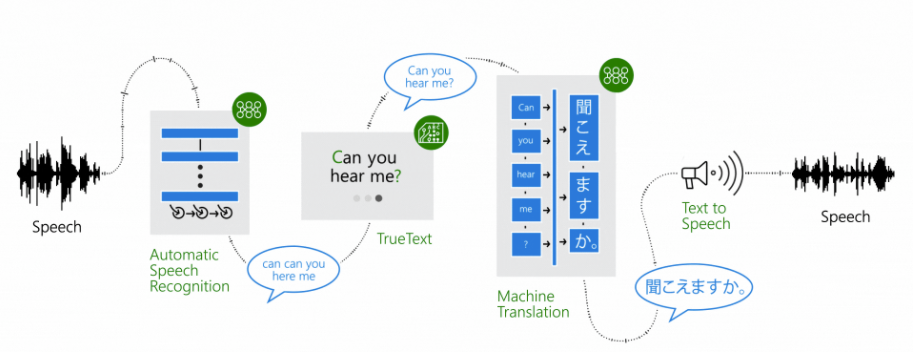
\includegraphics[width=\textwidth]{audiotrans.png}
    \caption{Real-time speech translation}
\end{figure}

\newpage
\section{Methodology}
Audio Translation mainly includes two steps: Speech Recognition, using Automatic Speech Recognition System (ASR) and Machine Translation.

\textbf{Automatic Speech Translation:} In this project, Whisper AI (from Open AI) is used which is an Automatic Speech Translation system. It has been trained on a large dataset of more than 650k hours of speeches of different people with different languages and accents.

\begin{figure}[!htb]
    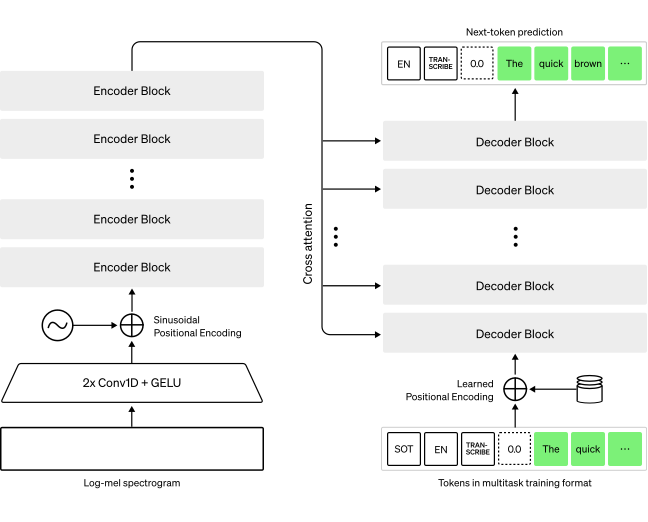
\includegraphics[width=\textwidth]{whisper1.png}
    \caption{Architecture of Whisper AI}
\end{figure}

The Whisper architecture is a simple end-to-end approach. It is implemented as an encoder-decoder Transformer where the input audio is split into 30-second chunks (parts), then converted into a log-Mel spectrogram, and atlast, it is passed into an encoder. A decoder is trained to predict the corresponding text caption which performs the processing along with the steps like, intermixing of special tokens that direct the single model to perform tasks such as language identification, phrase-level timestamps, multilingual speech transcription, and Translation of speech to English language.

\begin{figure}[!htb]
    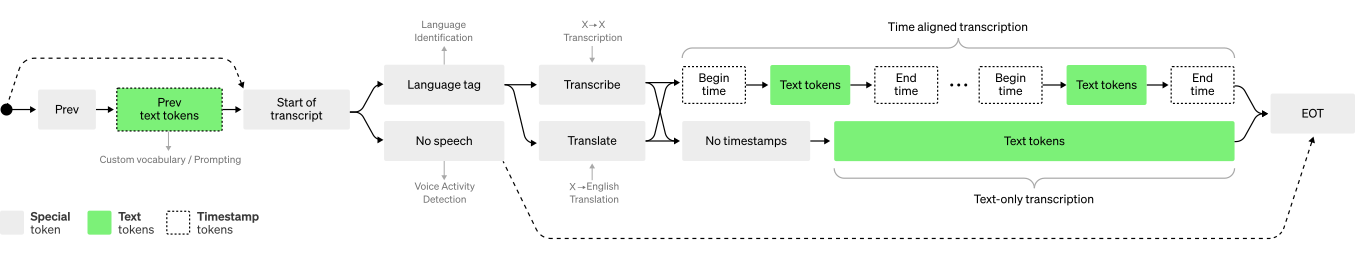
\includegraphics[width=\textwidth]{asr-details.png}
    \caption{Working of Automatic Speech Recognition(ASR)}
\end{figure}

\textbf{Machine Translation (MT):}
Machine Translation is the study of how to use computers to translate from one language into another. This concept was first put forward by Warren Weaver in 1947, just one year after the first computer, electronic numerical integrator and computer, was developed. At the same time, MT has been considered to be one of the most challenging tasks in the field of natural language processing (NLP). There are different approaches for machine translation ranging from rule-based to statistical to neural-based. Recently, more types of architectures like encoder-decoder attention-based architectures e.g., BERT have attained major improvements in machine translation. The WMT family of datasets is one of the most popular datasets used to benchmark machine translation systems. Some of the most commonly used evaluation metrics for machine translation systems include BLEU, METEOR, NIST, and others. The graphics below illustrate the overview of the working of Machine Translation: 

\begin{figure}[!htb]
    \centering
    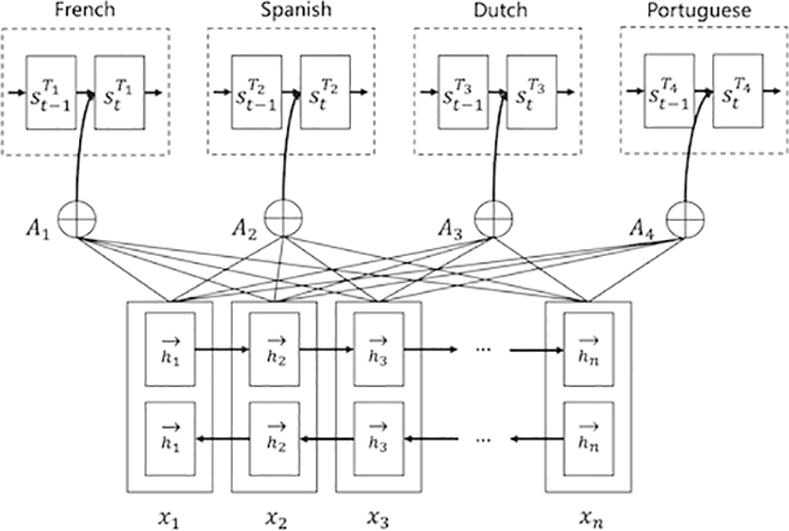
\includegraphics[width=\textwidth]{MT.jpg}
    \caption{Graphical abstract of Machine Translation}
\end{figure}

\section{Results and Discussion}
\textbf{Google Translator AI:}
    Google Translate leverages artificial intelligence (AI) in two key areas: machine translation (MT) and automatic speech recognition (ASR) for translating both text and speech. Here's a breakdown of how it works:

    \textbf{Machine Translation (MT):}

    Training on Massive Datasets: Google Translate is trained on vast amounts of parallel text data, where each piece of text has a corresponding translation in another language. This data comes from various sources like public web documents, books, and movie subtitles.

    \textbf{Statistical vs. Neural Approaches:} Traditionally, Google Translate used statistical models to analyze patterns in the training data and translate accordingly. However, in recent years, it has transitioned to more powerful neural machine translation (NMT) models.

    \textbf{Neural Networks for Complexities:} NMT models use artificial neural networks, similar to the structure of the human brain, to understand the relationships between words, phrases, and sentence structures across languages. This allows them to handle complex nuances and context-dependent translations.

    \textbf{Encoder-Decoder Architecture:}  NMT models typically have an encoder-decoder architecture. The encoder processes the source language text, capturing its meaning. The decoder then uses that information to generate the translated text in the target language.

    \textbf{Automatic Speech Recognition (ASR):}
    Speech-to-Text Conversion: This initial step involves converting the spoken audio into text. ASR models analyze the sound waves of the speech, recognizing phonemes (basic units of sound) and piecing them together to form words and sentences.

    \textbf{Deep Learning for Accuracy:}  Deep learning models play a crucial role in ASR. They are trained on large amounts of audio data with corresponding transcripts, allowing them to identify and distinguish various speech patterns, accents, and background noises.

    \textbf{Integration with MT:} Once the speech is converted to text, Google Translate's MT system takes over, translating the text from the source language to the target language as described earlier.

    \subsection{Accuracy levels of Google Translate for different target languages from English source content:}

    While Google Translate doesn't publish official accuracy ratings, various studies and benchmarks offer insights into its performance:

    \textbf{Success Stories:}

    \textbf{Major Languages:} Studies suggest Google Translate achieves accuracy exceeding 90\% for common phrases and documents between popular languages like English, Spanish, French, and Mandarin Chinese.

    \textbf{Academic Benchmarking:} The BLEU score, a common metric for evaluating machine translation, shows Google Translate reaching scores in the mid-to-high 80s for translating news articles between these major languages.
    Challenges and Considerations:

    \textbf{Less Common Languages:} Accuracy can drop significantly for languages with less training data. Research suggests a range of 60-80\% accuracy for some less common languages.

    \textbf{Beyond Basic Phrases:} For complex sentences or nuanced content, accuracy can fall below 80\%.

    \textbf{Domain-Specific Language:} Technical documents, legal jargon, or creative writing pose a particular challenge, with accuracy potentially dipping below 70\%.

\begin{table}[!h]
    \centering
    \begin{tabular}{|c|c|c|c|c|c|}
        \hline
        \multicolumn{2}{|c|}{\textbf{Accuracy levels of Google Translate for different target languages from English source content}} \\
        \hline

        Spanish & 94\% accurate\\
        \hline
        Korean & 82.5\% accurate\\
        \hline
        Mandarin Chinese & 81.7\% accurate\\
        \hline
        Farsi & 67.5\% accurate\\
        \hline
        Armenian & 55\% accurate\\
        \hline

    \end{tabular}
    \caption{Accuracy levels of Google Translate for different target languages from English source content}
\end{table}

\subsection{Available models and languages in Whisper AI and the Accuracy:}
There are five model sizes, four of which are English-only versions which offer speed and accuracy tradeoffs. Below are the names of the available models and their approximate memory requirements and inference speed relative to the large model. Actual speed may vary depending on many factors like the available hardware etc.

\begin{table}[!h]
    \centering
    \begin{tabular}{|c|c|c|c|c|c|}
        \hline
        \textbf{Size} & \textbf{Parameters} & \textbf{English-only model} & \textbf{Multilingual model} & \textbf{Required VRAM} & \textbf{Relative speed}\\
        \hline
        tiny & 39 M & tiny.en & tiny & ~1 GB & ~32x\\
        \hline
        base & 74 M & base.en & base & ~1 GB & ~16x\\
        \hline
        small & 244 M & small.en & small & ~2 GB & ~6x\\
        \hline
        medium & 769 M & medium.en & medium & ~5 GB & ~2x\\
        \hline
        large & 1550 M & N/A & large & ~10 GB & 1x\\
        \hline

    \end{tabular}
    \caption{Available models and languages in Whisper AI}
\end{table}


The .en models from the above mentioned models in Table. 1 tend to perform better for English-only applications, especially for the tiny.en and base.en models. It has been observed by the Whisper AI developers that the difference in performance becomes less significant for the small.en and medium.en models.

The performance of the Whisper model varies widely depending on the language used. The figure below shows a performance breakdown of large-v3 and large-v2 models by language, using WERs (word error rates) or CER (character error rates, shown in Italic) evaluated on the Common Voice 15 and Fleurs datasets. 

\pagebreak
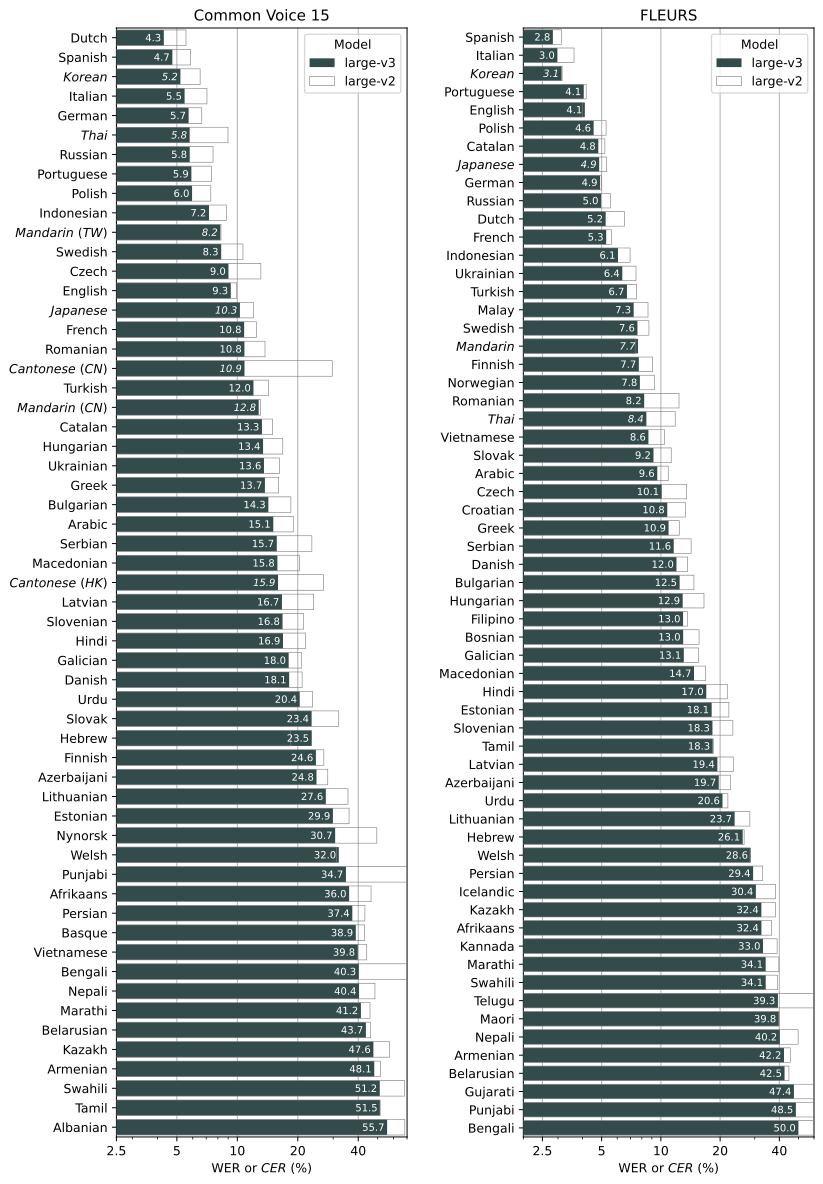
\includegraphics[width=\textwidth]{wer-cer.png}

\section{Future Scope}
Preserving accents in real-time audio translation (RT-ATT) offers a compelling avenue for enhancing user experience and fostering natural communication. While the proposed approach presents a promising initial step, several exciting directions can be explored to further refine and extend its capabilities.

\textbf{Accent Recognition and Normalization:}
Improved Accent Embeddings: The current approach relies on embedding techniques to capture accent information. Future work could involve investigating more sophisticated methods like speaker diarisation or end-to-end accent-aware models to create even richer accent representations.

\textbf{Accent Normalization for Fluency:} While preserving accents is desirable, extreme cases might lead to reduced fluency in the target language. Future research could explore normalization techniques that mitigate strong accents while retaining some speaker characteristics, achieving a balance between fidelity and naturalness.

\textbf{Multi-speaker and Background Noise Handling:}
Speaker Separation for Group Conversations: Real-world scenarios often involve multiple speakers with different accents. The current approach can be extended to incorporate speaker separation techniques to isolate individual voices and preserve their unique accent characteristics during translation.

\textbf{Background Noise Reduction with Accent Awareness:} Background noise can significantly impact accent recognition. Future work could explore noise reduction methods specifically tailored for audio with accents, ensuring fidelity is maintained even in challenging listening environments.

\textbf{User Preferences and Control:}

\textbf{Dynamic Accent Control:} Users might desire varying levels of accent preservation depending on the context. The system could be enhanced to allow users to dynamically adjust the degree of accent preservation based on their preferences.

\textbf{Accent Adaptation:} The system could be equipped with the ability to adapt its translation style to match the target audience's preferences. For instance, translating for a multilingual audience might involve toning down strong accents for better comprehension.

\textbf{Exploration of New Applications:}
Language Learning Applications: RT-ATT with accent preservation can be a valuable tool for language learners, allowing them to practice listening comprehension with various accents and enriching their exposure to the target language.
Multilingual Customer Service: Businesses catering to a global audience can leverage this technology to provide more natural and culturally sensitive customer service interactions, preserving the nuances of communication across languages.

\textbf{Explainable AI and Trustworthiness:}

\textbf{Understanding Accent-based Errors:} Developing methods to explain how the system translates accented speech can be crucial. This can help users understand potential errors or inconsistencies arising from accent recognition or preservation techniques.

\textbf{Combating Bias:} Accented speech can be correlated with certain demographics. Future work should explore methods to mitigate bias in accent recognition and translation, ensuring fair and inclusive performance across different speaker populations.
By addressing these future directions, researchers can significantly enhance the capabilities of RT-ATT with accent preservation. This technology has the potential to revolutionize communication, fostering genuine human connection and mutual understanding across languages and cultures.

\section{Conclusion}
The preservation of accents in real-time audio translation (RT-ATT) represents a giant leap towards a future of inclusive and nuanced communication. The proposed approach lays a strong foundation, but the journey continues. By venturing into the exciting realms outlined in the future scope, researchers can unlock a new generation of RT-ATT systems. Imagine a world where:

\textbf{Language learning flourishes:} Learners can immerse themselves in the richness of diverse accents, honing their comprehension skills and appreciating the cultural tapestry of a language.

\textbf{Global businesses thrive:} Customer interactions transcend language barriers, fostering trust and connection through accent-aware translations that respect individual voices.
Real-time conversations flow effortlessly: At conferences, meetings, or on the street, multilingual discussions unfold naturally, preserving the speaker's essence while ensuring clear understanding.
This vision hinges not only on technological advancements but also on responsible development. Explainable AI techniques will empower users to understand the system's reasoning, fostering trust and transparency. Combating bias in accent recognition and translation will ensure fair and inclusive performance for all speaker demographics.
The path ahead is paved with exciting challenges and immense potential. As we continue to refine RT-ATT with accent preservation, we pave the way for a future where communication transcends language, celebrates individuality, and fosters a deeper understanding between people across the globe. This technology holds the power to break down walls, build bridges, and create a world where everyone can be heard, understood, and valued in their unique voice.


\section{References}
\begin{enumerate}
    \item Jinyu Li - Recent Advances in End-to-End Automatic Speech Recognition [https://arxiv.org/abs/2111.01690]
    \item Whisper AI [https://github.com/openai/whisper]
    \item Alec Radford, Jong Wook Kim, Tao Xu,  Greg Brockman,  Christine McLeavey, Ilya Sutskever - Robust Speech Recognition via Large-Scale Weak Supervision [https://arxiv.org/pdf/2212.04356.pdf]
    \item Jiahuan Li, Shanbo Cheng, Shujian Huang, Jiajun Chen - MT-PATCHER: Selective and Extendable Knowledge Distillation from Large Language Models for Machine Translation [https://arxiv.org/abs/2403.09522/]
    \item Dzmitry Bahdanau, Kyunghyun Cho, Yoshua Bengio - Neural Machine Translation by Jointly Learning to Align and Translate
    [https://arxiv.org/abs/1409.0473/]
\end{enumerate}
\end{document}